\documentclass[14pt, a4paper]{extarticle}
\title{1.8 Graphing Polynomial Functions}
\usepackage[a4paper, papersize={8.5in, 120in}, total={7.5in, 120in}]{geometry}
\usepackage{setspace}
\usepackage{amsmath}
\usepackage{amssymb}
\usepackage{changepage}
\usepackage{tikz}
\usepackage{pgfplots}
\usepackage{polynom}

\author{Jacob Zante}
\date{September 26th, 2024}
\doublespacing
\pgfplotsset{width=7in, compat=newest}
% \usepgfplotslibrary{external}

\begin{document}
\maketitle
\setlength{\parindent}{0pt}

\textbf{1. State the degree, leading coefficient, x-intercepts, and graph the following functions:} \\
\begin{adjustwidth}{1cm}{0pt}
    \textbf{a) $y = (x - 1)(x + 4)$} \\
    x-ints: $x = 1:$: order 1, $x = -4$: order 1 \\
    degree: 2 \\
    leading coefficient: +
    \begin{adjustwidth}{-1cm}{0pt}
        \begin{tikzpicture}
            \begin{axis}[
                axis lines=middle,
                axis line style={thick,<->},
                xmin=-10,xmax=10,ymin=-10,ymax=10,
                ytick={-10,-8,...,+10},
                xtick={-10,-8,...,+10},
                tick label style={font=\normalsize},
                grid=major,
                major grid style={dashed,very thin,black},
                every axis plot post/.append style={thick},
                label style={font=\normalsize},
                % x label style={at={(axis description cs:0.5,-0.05)},anchor=north},
                % y label style={at={(axis description cs:-0.05,0.5)},rotate=90,anchor=south},
                xlabel=$x$,
                ylabel=$y$,
                smooth,
                legend style={
                        font=\normalsize,
                        at={(0.5, 1.1)},
                        anchor=north
                        }
                ]
                \addplot[domain=-10:10,samples=200,blue]{(x - 1)*(x + 4)};
                \legend{$y = (x - 1)(x + 4)$}
            \end{axis}
        \end{tikzpicture}
    \end{adjustwidth}
    \textbf{b) $y = -(x - 1)^3(x + 4)(x - 5)^2$} \\
    x-ints: $x = 1$: order 3, $x = -4$: order 1, $x = 5$: order 2 \\
    degree: 6 \\
    leading coefficient: -
    \begin{adjustwidth}{-1cm}{0pt}
        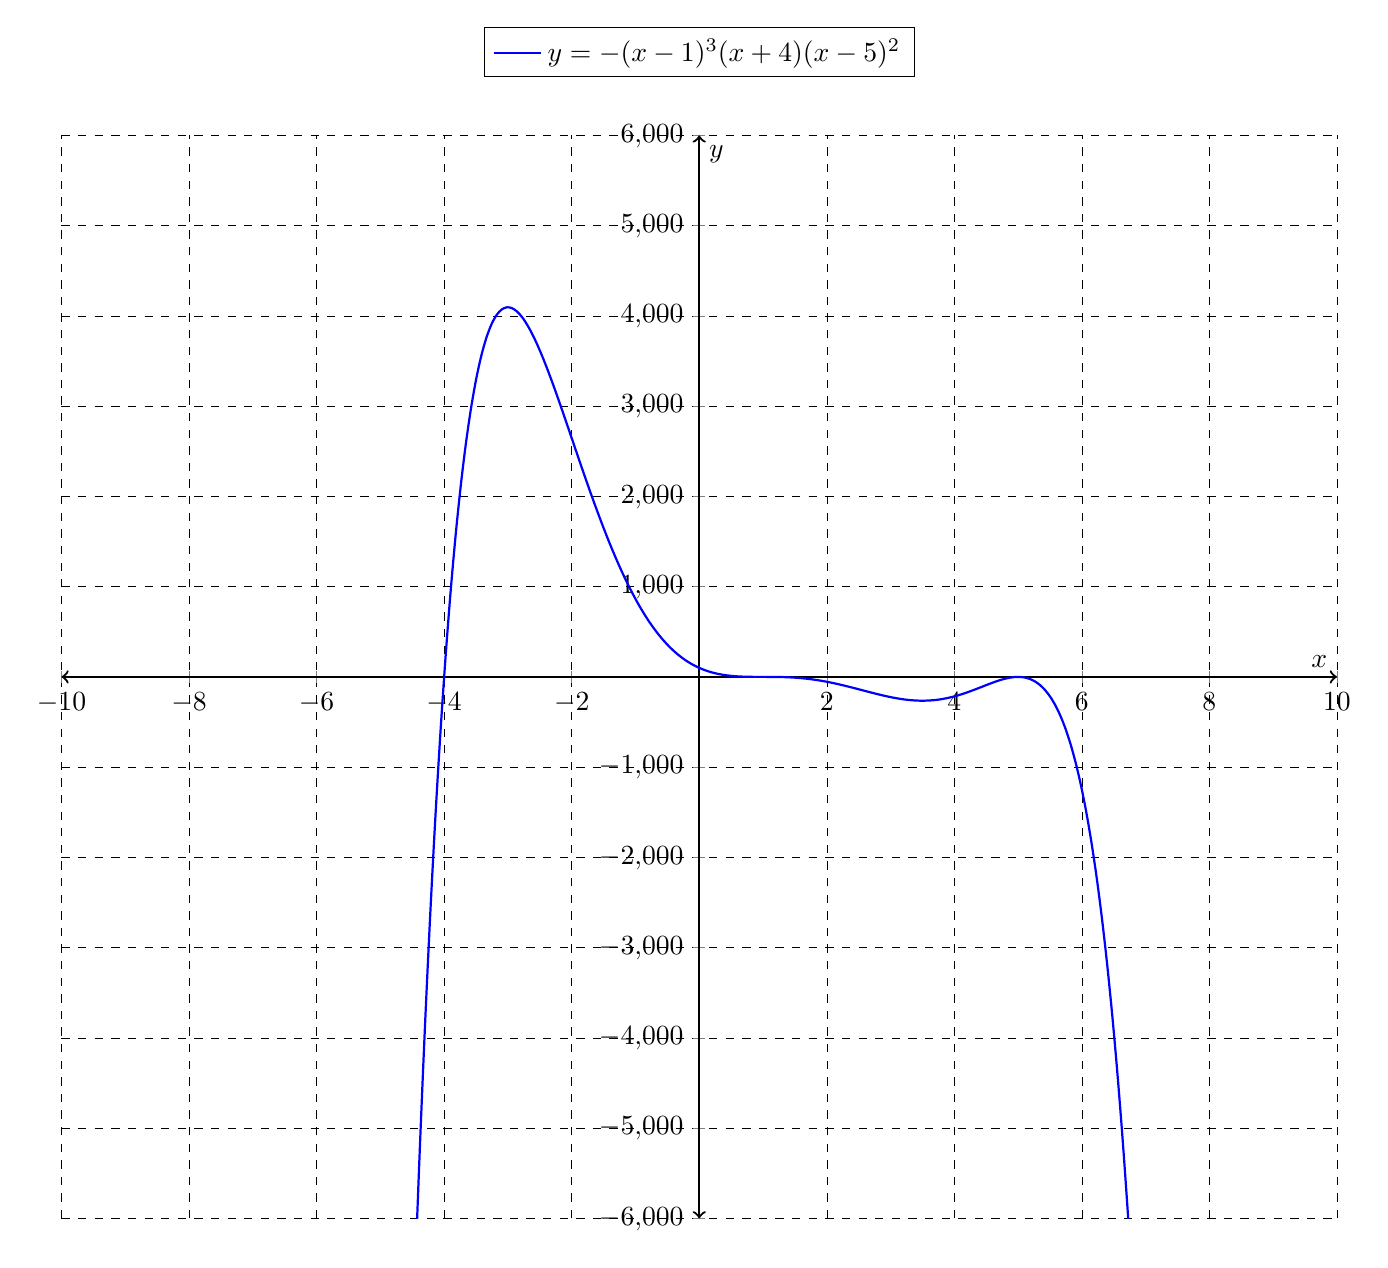
\begin{tikzpicture}
            \begin{axis}[
                axis lines=middle,
                axis line style={thick,<->},
                xmin=-10,xmax=10,ymin=-6000,ymax=6000,
                ytick={-6000,-5000,...,+6000},
                xtick={-10,-8,...,+10},
                tick label style={font=\normalsize},
                grid=major,
                major grid style={dashed,very thin,black},
                every axis plot post/.append style={thick},
                label style={font=\normalsize},
                % x label style={at={(axis description cs:0.5,-0.05)},anchor=north},
                % y label style={at={(axis description cs:-0.05,0.5)},rotate=90,anchor=south},
                xlabel=$x$,
                ylabel=$y$,
                smooth,
                legend style={
                        font=\normalsize,
                        at={(0.5, 1.1)},
                        anchor=north
                        }
                ]
                \addplot[domain=-8:8,samples=200,blue]{-1 * (x - 1)^3 * (x + 4) * (x - 5)^2};
                \legend{$y = -(x - 1)^3(x + 4)(x - 5)^2$}
            \end{axis}
        \end{tikzpicture}
    \end{adjustwidth}
    \textbf{c) $y = (x + 3)^2(x - 2)^2(x + 1)^3(x + 5)$} \\
    x-ints: $x = -3$: order 2, $x = 2$: order 2, $x = -1$: order 3, $x = -5$: order 1 \\
    degree: 8 \\
    leading coefficient: +
    \begin{adjustwidth}{-1cm}{0pt}
        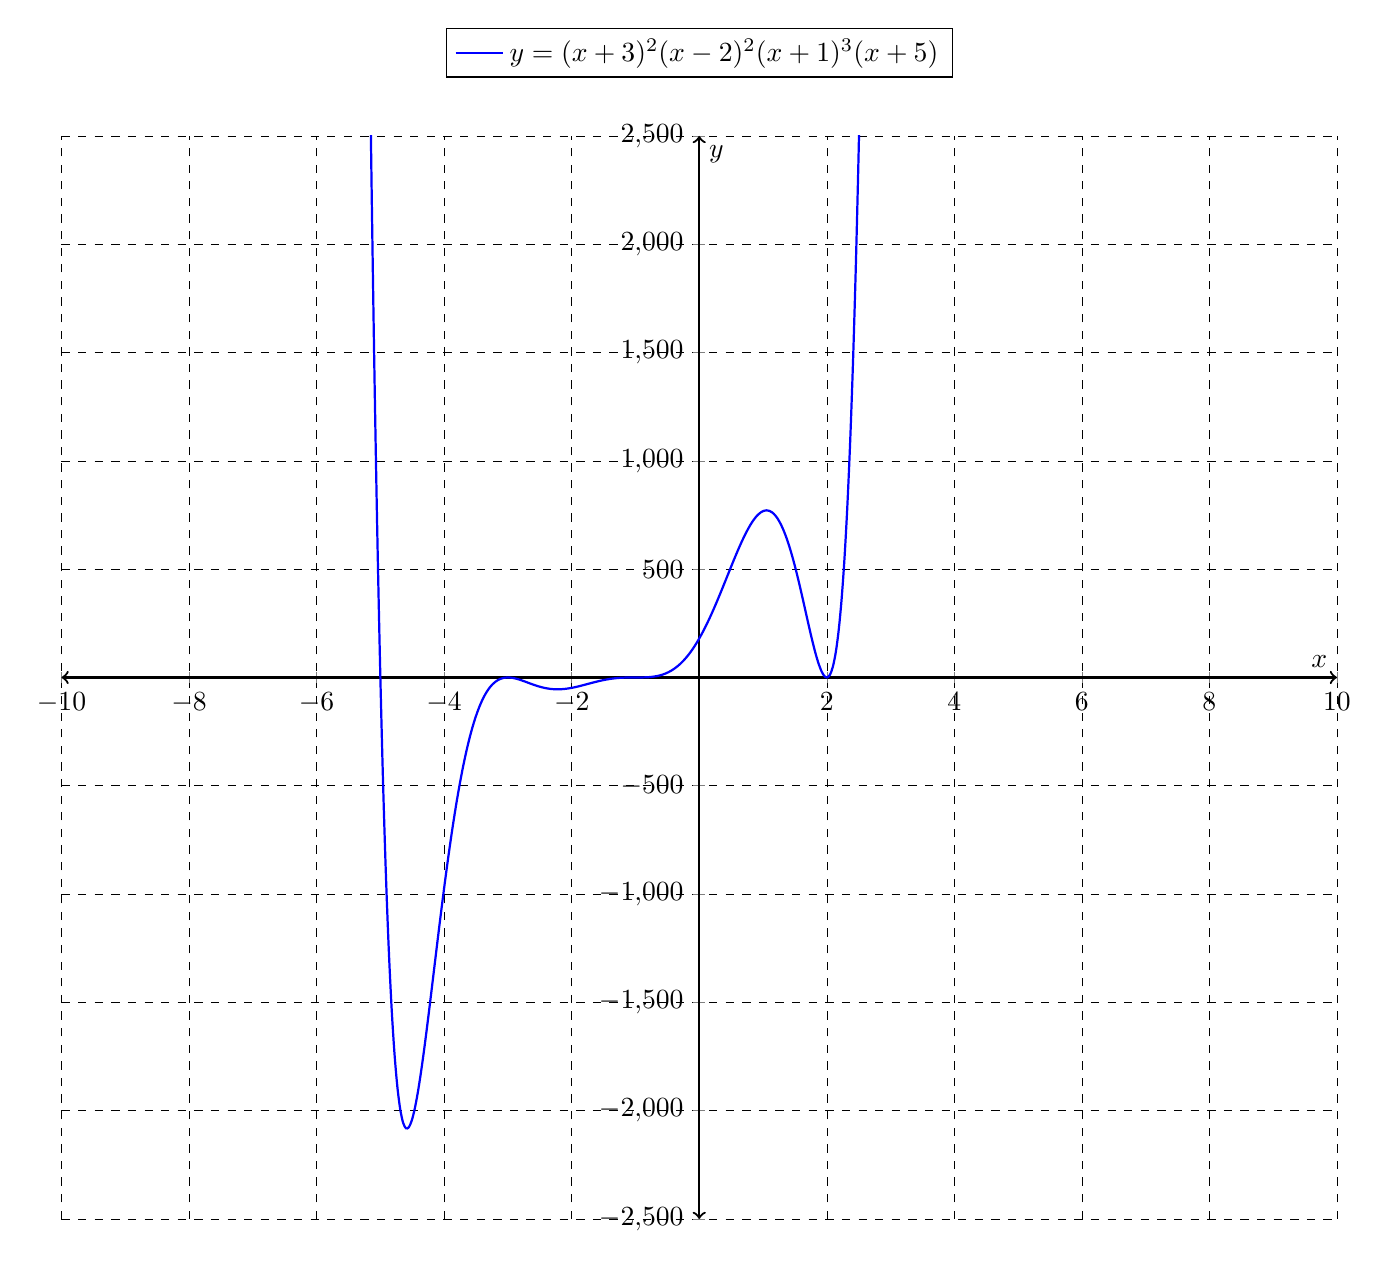
\begin{tikzpicture}
            \begin{axis}[
                axis lines=middle,
                axis line style={thick,<->},
                xmin=-10,xmax=10,ymin=-2500,ymax=2500,
                ytick={-2500,-2000,...,+2500},
                xtick={-10,-8,...,+10},
                tick label style={font=\normalsize},
                grid=major,
                major grid style={dashed,very thin,black},
                every axis plot post/.append style={thick},
                label style={font=\normalsize},
                % x label style={at={(axis description cs:0.5,-0.05)},anchor=north},
                % y label style={at={(axis description cs:-0.05,0.5)},rotate=90,anchor=south},
                xlabel=$x$,
                ylabel=$y$,
                smooth,
                legend style={
                        font=\normalsize,
                        at={(0.5, 1.1)},
                        anchor=north
                        }
                ]
                \addplot[domain=-6:3,samples=200,blue]{(x + 3)^2 * (x - 2)^2 * (x + 1)^3 * (x + 5)};
                \legend{$y = (x + 3)^2(x - 2)^2(x + 1)^3(x + 5)$}
            \end{axis}
        \end{tikzpicture}
    \end{adjustwidth}
    \textbf{d) $y = x^2(x - 3)^2$} \\
    x-ints: $x = 0$: order 2, $x = 3$: order 2 \\
    degree: 4 \\
    leading coefficient: +
    \begin{adjustwidth}{-1cm}{0pt}
        \begin{tikzpicture}
            \begin{axis}[
                axis lines=middle,
                axis line style={thick,<->},
                xmin=-10,xmax=10,ymin=-20,ymax=20,
                ytick={-20,-15,...,+20},
                xtick={-10,-8,...,+10},
                tick label style={font=\normalsize},
                grid=major,
                major grid style={dashed,very thin,black},
                every axis plot post/.append style={thick},
                label style={font=\normalsize},
                % x label style={at={(axis description cs:0.5,-0.05)},anchor=north},
                % y label style={at={(axis description cs:-0.05,0.5)},rotate=90,anchor=south},
                xlabel=$x$,
                ylabel=$y$,
                smooth,
                legend style={
                        font=\normalsize,
                        at={(0.5, 1.1)},
                        anchor=north
                        }
                ]
                \addplot[domain=-2:5,samples=200,blue]{x^2 * (x - 3)^2};
                \legend{$y = x^2(x - 3)^2$}
            \end{axis}
        \end{tikzpicture}
    \end{adjustwidth}
    \textbf{e) $y = (x - 2)^3(x + 1)(x + 5)^2$} \\
    \\
    \textbf{f) $y = (x - 2)^2(x + 2)^2$} \\
\end{adjustwidth}


\end{document}